\section{Design Principles}

\sys follows three key design principles:

\paragraph{Principle 1: Transparent and Dynamically Programmable GPU OS Interface.}
Userspace policies hard to provide transparent or robust control across rapidly evolving and diverse GPU applications. \sys therefore embeds dynamically programmable, transparent policy interfaces at the GPU OS and driver layers, using lightweight dynamic binary instrumentation for device code and enable seamless policy evolution.

\paragraph{Principle 2: Single Programming and Execution Model Across Host and GPU.}
Fragmented CPU–GPU policy models complicate coordination and lead to inconsistent resource-management behavior. \sys unifies host and GPU policy execution under a single programming abstraction and control plane, simplifying policy expression and enabling coherent, cross-layer decisions.

\paragraph{Principle 3: SIMT-Aware Load-Time Verification and Optimization.}
GPU SIMT execution fundamentally diverges from scalar CPU semantics, making traditional eBPF verification insufficient and runtime isolation prohibitively expensive on resource-constrained GPUs. \sys introduces load-time SIMT‑aware verification and optimization to ensure safe execution, bounded resource usage, predictable latency, and minimal runtime overhead.

\section{\sys Design}

\subsection{High-Level Architecture}
\label{sec:arch}

\begin{figure}
\centering
    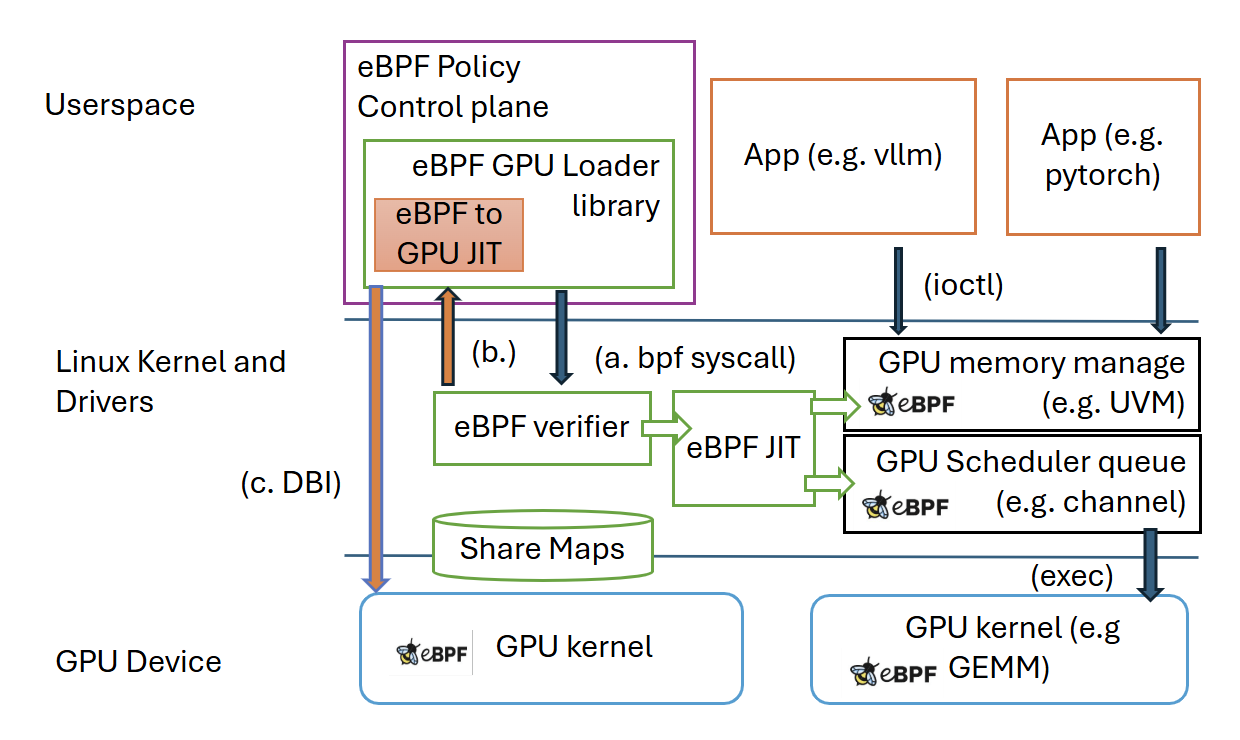
\includegraphics[width=\columnwidth]{img/gpu-ebpf-arch.png}
\vspace{-.5ex}
\caption{\sys high-level design: unified eBPF runtime spanning CPU and GPU.}
\label{fig:system-design}
\end{figure}

Figure~\ref{fig:system-design} shows the high-level architecture of \sys, composed of a user-space control plane and a unified kernel-and device-side execution path. policies in \sys consist of coordinated host- and device-side eBPF programs, hierarchical cross-layer maps, and a user-space control plane for lifecycle management.

\sys exposes \emph{hierarchical cross-layer maps}: logical eBPF map abstractions whose backing storage is automatically partitioned and replicated across host DRAM, GPU global memory, and optionally per-SM scratch space, with consistency and placement managed transparently by the runtime. Policy developers access maps via standard eBPF helpers regardless of execution context, without manual DMA transfers, memory placement, or address translation.

\paragraph{User-space Control Plane.}
Policy authors use standard eBPF tooling (e.g., \texttt{clang/libbpf}, \texttt{bpftool}) to build policy bytecode. The control-plane links against a loader library that installs policies and configures hierarchical maps. It enables runtime policy redeployment and reconfiguration (e.g., eviction thresholds, sampling rates, priorities) without application or kernel restarts, and exports runtime metrics (e.g., region hotness, tenant latencies) to external systems.

\paragraph{Kernel and Device Runtime.}
\sys provides a unified runtime across kernel and GPU contexts, managing verification, compilation, and map placement. It employs a SIMT-aware verifier (\S\ref{sec:verification}) that extends standard eBPF checks to reason about warp-uniformity, SIMT control flow, and GPU synchronization constraints. Verified programs are JIT-compiled into native host code or GPU-compatible instructions (e.g., PTX). The runtime manages hierarchical cross-layer maps as described above, dynamically optimizing placement based on access patterns and capacity constraints.

Policy execution occurs at structured hook points defined in GPU drivers and kernels. On the host, \sysdriver exposes \texttt{struct\_ops}-style hooks (e.g., region admission/eviction, kernel scheduling). Host handlers return concise policy decisions enforced via trusted kfuncs. On the GPU device, \sys injects lightweight trampolines at kernel entry/exit, warp synchronization barriers, and critical memory operations, invoking device-side handlers at warp granularity. Device handlers update cross-layer maps with performance signals (e.g., region access patterns, warp occupancy) and make granular control decisions (e.g., prefetch hints, block-level scheduling). Handlers never directly manipulate hardware registers or page tables; instead, they issue policy decisions via trusted helpers and kfuncs that the runtime enforces. GPU device eBPF also has access to general helpers like get time stamps.

\subsection{Challenges}
\label{sec:challenges}
\xiangyu{This section is updated.}
Achieving programmable resource management on GPUs remains fundamentally difficult today. 
Unlike CPUs—where extension frameworks such as eBPF provide stable, safe, and well-defined programmability points—GPU software stacks were not designed with similar goals. 
We identify three core challenges that make GPU programmability hard.

\subsubsection{C1: Lack of Safe and Stable Extension Points in Monolithic GPU Drivers}
Modern GPU drivers are large, monolithic vendor-controlled codebases that tightly intertwine low-level hardware mechanisms with proprietary resource-management policies, offering no stable hooks for user-defined logic. 
GPU drivers were not architected with programmable resource management in mind—partly due to historical assumptions about GPU usage, and partly due to strict safety constraints, as incorrect driver logic can stall the device or crash an entire node. 
As a result, developers cannot inject new scheduling policies, memory-placement strategies, or custom instrumentation without invasive modifications to vendor drivers. This absence of safe, stable extension points naturally limits any attempt to retrofit programmability into today's GPU stacks.

\subsubsection{C2: Mismatch Between CPU Extension Semantics and the SIMT GPU Execution Model}

\yusheng{mismatch between verify extension single thread CPU model vs SIMT GPU model, kernel concurrency / extension, not eBPF Semantics}

Even if GPU drivers exposed extensible interfaces, directly applying existing programmable CPU-oriented eBPF mechanisms does not work because of the conflict between eBPF semantics and the GPU Single Instruction Multiple Threads (SIMT) execution model execution model. 
Concretely, eBPF programs assume single-threaded control flow, strong memory consistency, and bounded execution enforced by a CPU-oriented verifier, whereas GPU kernels execute in warps of 32 threads that must follow largely uniform control paths. 
Naively running scalar eBPF logic per thread introduces warp divergence, unbounded serialization, and correctness risks stemming from thousands of simultaneous memory operations that the CPU-side verifier do not check. 
Furthermore, GPUs lack isolation, recovery points, or preemption mechanisms for misbehaving device-side code, meaning an unbounded loop or invalid access in policy logic can halt an entire device. 
The architectural and semantic mismatch makes straightforward reuse of eBPF unsafe and inevitably slow.

\subsubsection{C3: Absence of Efficient Mechanisms for Host–Device Shared State Status}

Even with GPU-side programmability that respects SIMT constraints, real GPU clusters require coordinated host–device resource management, which today lacks an efficient abstraction for shared policy state. 
GPU-accessible host memory suffers from orders-of-magnitude higher latency than GPU global memory, while GPU memory is capacity-limited and optimized for throughput, creating a fundamental mismatch in memory hierarchies. 
Meanwhile, CPU and GPU components operate asynchronously on vastly different timescales, causing policy decisions to rely on inconsistent state unless carefully synchronized. 
Existing systems force developers to manually manage DMA transfers, data replication, and consistency across devices, resulting in brittle, application-specific mechanisms that do not generalize.
The absence of a principled, efficient way to maintain shared state across the host–device boundary remains a major barrier to deploying practical programmable resource management on GPU clusters.


\subsection{\sys{} Policy Interfaces}
\label{sec:design-interfaces}

\sys introduces three eBPF program types for GPU resource management: two driver‑level types, \texttt{BPF\_PROG\_TYPE\_GPU\_MEM} for memory‑placement policy and \texttt{BPF\_PROG\_TYPE\_GPU\_SCHED} for scheduling decisions, and one device‑level type, \texttt{BPF\_PROG\_TYPE\_GPU\_DEV}, for in‑kernel GPU instrumentation. These program types coexist with existing kernel eBPF program types and are distinguished solely by their attach points and their SIMT‑specific verification rules.

\subsubsection{Memory Interface}
\label{sec:design-mem}

\sys treats memory placement as a programmable region cache. It exposes four region-level events (\emph{add}, \emph{access}, \emph{removal}, and \emph{prefetch}) and allows host and device policies to cooperate. \sys regions correspond directly to GPU hardware-managed units, such as 2MB physical UVM chunks or VA blocks, and finer-grained 4KB pages. This granularity balances fine-grained memory behavior against the prohibitive overhead of per-page metadata, enabling efficient policy decisions closely aligned with underlying GPU hardware. Additionally, using regions as a logical abstraction allows \sys to transparently hide diverse vendor-specific and driver-level complexities, providing a uniform, programmable interface. The host driver exports these events through a small \texttt{struct\_ops} table. Handlers encode decisions through an enum field in the context and may reorder—but never remove—regions in the kernel‑maintained eviction list. The kernel always enforces safety and correctness, including fallback FIFO eviction under pressure. Policies maintain their own metadata in hierarchical maps and express placement and prefetch decisions through these callbacks. Device‑side kernels observe memory operations and express future‑use hints through a device‑level interface. Device handlers receive a compact warp‑uniform context and operate at warp granularity. Operation like prefetch can be performed on device and then trigger host-side prefetch callbacks, enabling the host to combine cross‑kernel information with device‑side predictive logic.


\begin{minted}[
    highlightlines=false,
    fontsize=\footnotesize,
    breaklines=true,        % 开启自动换行
    breaksymbolleft=,       % 【关键】去除换行处的箭头符号
    breakindent=1em,        % 换行后缩进 1em，视觉上区分
    baselinestretch=0.9
]{c}
// Host-side policy callbacks for GPU memory management
struct gdrv_mem_ops {
  // Region created or eligible for device placement
  int (*region_add)(gdrv_mem_add_ctx_t *ctx);
  // Memory subsystem observes region use;
  // decide cache hit/eviction policies
  int (*region_access)(gdrv_mem_access_ctx_t *ctx);
  // Region about to leave device-resident working set
  int (*region_remove)(gdrv_mem_remove_ctx_t *ctx);
  // Safe points (kernel launches, faults) for prefetch
  int (*prefetch)(gdrv_mem_prefetch_ctx_t *ctx);
};

// Host-side kfuncs: reorder regions in eviction list
bool gdrv_mem_list_insert_head(gdrv_mem_list_t *list,
                               gmem_region_t *r);
bool gdrv_mem_list_insert_tail(gdrv_mem_list_t *list,
                               gmem_region_t *r);

// Device-side memory callback interface
struct gdev_mem_ops {
    // Warp observed memory access;
    void (*access)(gdev_mem_access_ctx_t *ctx);
    // Kernel provides
    void (*fence)(gdev_mem_fence_ctx_t *ctx);
};

// Device-side helpers
// Request prefetch, triggers callback in kernel
 int gdev_mem_prefetch(gmem_region_t* r);
\end{minted}

% map(address)

% // hostside
% prefetch_callback() {
% // check logic
%     prefetch region(device,address)
% }

% //device side
% SEC(gdev_entry/xxx)
% ebpf_gpu(int expert_id) {
%     gdev_mem_use_hint（address a, b)
% }
% // Pin memory on CPU or GPU
%  int gdev_mem_pin_hint(gmem_region_t* r, int dev_id);
% int gdev_mem_use_hint(gmem_region_t* r, int dev_id);

\subsubsection{Scheduling Interface}
\label{sec:design-sched}

\sys exposes policy control at two levels: hardware‑queue lifecycle (host‑side) and thread‑block scheduling (device‑side). The host participates in GPU queue admission and priority control through Policies set queue priority, timeslice, and may reject or defer queue creation, enabling true admission control. Properties are written directly into firmware‑visible structures, ensuring enforcement beyond user‑space hints. Policies may also invoke the \texttt{gdrv\_sched\_preempt} kfunc to trigger cooperative preemption through the driver’s native context‑switch mechanism.

Within the GPU, \sys provides a work‑stealing thread‑block scheduler. Kernels expose their logical work units; persistent worker blocks select and process units while device‑side eBPF handlers steer scheduling decisions via \texttt{gdev\_block\_ctx}. The verifier ensures that scheduling decisions respect kernel invariants (e.g., selecting only local work units). \sys can inject this scheduler via binary rewriting or allow developers to integrate it explicitly.

\begin{minted}[highlightlines=false,fontsize=\footnotesize]{c}
// Host-side policy callbacks for GPU hardware
// queue scheduling
struct gdrv_sched_ops {
  // Hardware queue creation; set prio/timeslice,
  // return 0 to accept or <0 to reject/defer
  int  (*queue_create)(gsched_queue_ctx_t *ctx);
  // Hardware queue destruction; cleanup policy
  void (*queue_destroy)(gsched_queue_ctx_t *ctx);
};

// Host-side kfunc
bool gdrv_sched_preempt(gdrv_preempt_ctx_t *ctx);

// Device-side block scheduling callbacks
struct gdev_sched_ops {
  // Worker block starts/exits new work unit
  void (*enter)(gdev_block_ctx_t *ctx);
  void (*exit)(gdev_block_ctx_t *ctx);
  
  // Device function starts/ends
  void (*probe)(gdev_block_ctx_t *ctx);
  void (*retprobe)(gdev_block_ctx_t *ctx);
  
  // Return whether to steal work (TB scheduler)
  bool (*should_try_steal)(gdev_block_ctx_t *ctx);
};
\end{minted}

\subsection{Runtime Verification and Optimizations}
\label{sec:verification}

\sys policies execute directly within privileged GPU driver and kernel contexts, making strong safety guarantees essential. We adopt a standard eBPF threat model: we trust cluster operators loading policies, but consider policy code potentially buggy or misconfigured. The trusted computing base (TCB) includes the kernel eBPF verifier, \sys-specific kernel module, GPU runtime backend, and GPU driver/firmware. Policy authors only interact with eBPF abstractions and do not write native device code. For host-side verification, we reuse the existing Linux kernel eBPF verifier unchanged, relying on standard type-checking, bounded-loop, and memory-safety constraints. \sys-specific kfuncs and hooks are declared via BPF Type Format (BTF) metadata.

\subsubsection{SIMT-aware Verification (Design)}

Traditional scalar eBPF semantics hard be efficiently or safely executed directly in GPU SIMT contexts due to potential severe warp divergence, unsafe synchronization effects and unpredictable resource consumption. \sys introduces a novel SIMT-aware static verification model enforcing warp-level uniformity constraints to ensure efficient and safe GPU-side policy execution.

The key insight is that we explicitly distinguish \emph{warp-uniform} values (identical across warp threads, e.g., region identifiers) from \emph{lane-varying} values (thread-local GPU state). Policies may compute freely using lane-varying values, but these must not influence control-flow decisions or directly produce side effects visible outside a warp. To guarantee warp-level coherence, \sys mandates that branch conditions, loop bounds, and map-update keys be warp-uniform or derived via warp-level aggregation. Additionally, \sys explicitly prohibits GPU-wide barriers, global synchronization primitives, and non-uniform atomic operations, and imposes explicit resource budgets per policy hook to bound resource usage. These design constraints ensure that programmable policy logic can be safely integrated into privileged GPU contexts, adhering strictly to GPU hardware execution semantics.

\subsubsection{Warp-level Execution Optimizations}

Direct scalar execution of eBPF handlers on GPU threads would cause prohibitive warp divergence and excessive resource overhead. To resolve this, \sys introduces a warp-level aggregated execution model, executing policy logic exactly once per warp using a designated "warp leader" (typically lane 0). Each hook invocation conceptually follows a two-phase approach: each lane independently computes lane-local contributions (e.g., effective addresses, counters) without influencing control flow or directly updating shared state. These contributions are then aggregated at warp granularity. Subsequently, the warp leader executes the policy handler once using aggregated inputs and warp-uniform context. The resulting decision is broadcast back to all lanes. This design strictly eliminates divergence and minimizes GPU overhead while preserving eBPF's scalar semantics. To further reduce runtime overhead, \sys employs aggressive compiler-level optimizations (specialization and inlining) tailored specifically for warp-level execution.

\subsubsection{Hierarchical Cross-layer Maps for State Coordination}

Effective GPU policy decisions require coherent sharing of policy state across asynchronous CPU and GPU contexts. To transparently bridge CPU-GPU memory hierarchies, \sys introduces hierarchical cross-layer maps. Logically, each map is a single unified key-value store accessible from host-side driver hooks, GPU-side handlers, and user-space policy control planes, and verifiable through eBPF's existing model. Physically, maps are realized as hierarchical shards across host DRAM, GPU global memory, and GPU-local storage (e.g., shared memory, SM-local). The runtime dynamically determines shard placement based on access frequency, latency, and capacity constraints. Following eBPF's soft-state philosophy, \sys maps provide relaxed, eventual consistency. Instead of strong global ordering, our runtime periodically merges GPU-local map shards into canonical snapshots at well-defined synchronization points—typically GPU kernel completion boundaries. This snapshot-based model is sufficient for policy decisions relying on approximate statistics. Occasional staleness affects decision optimality but cannot violate correctness invariants such as memory integrity, which remain enforced by the GPU driver and hardware MMU.
